\documentclass[beamer=true]{standalone}
\usepackage{../../preamblesnotes}

%Information to be included in the title page:
\title{第五課}
\author{動量 I Momentum I}
\institute{全年班}
\date{}

\begin{document}
\frame{\titlepage}

% \begin{frame}{動量是什麼?What is momentum}

% \end{frame}

\begin{frame}{動量Momentum}
    \begin{itemize}
        \item 質量和速度的乘積
    \end{itemize}
    \begin{alertblock}
        {動量Momentum $\vec{p}$}
        \begin{equation}
            \vec{p}=m\vec{v}
        \end{equation}
    \end{alertblock}
    \begin{itemize}
        \item 動量是向量
        \item 單位Unit: [\unit{kg.m.s^{-1}}] or [\unit{N.s}]
    \end{itemize}
\end{frame}

\begin{frame}{動量改變Momentum change}
    動量的改變 $=$ 最終動量 $–$ 起始動量
    \begin{exampleblock}
        {動量的改變 $\Delta \vec{p}$}
        \begin{equation}
            \Delta\vec{p}=m\vec{v}-m\vec{u}
        \end{equation}
    \end{exampleblock}
\end{frame}

\begin{frame}{動量改變Momentum change}
    \begin{itemize}
        \item 要注意動量本身是有方向的:
        \item 例如,取向右的方向為正:
    \end{itemize}
    {\par\centering
    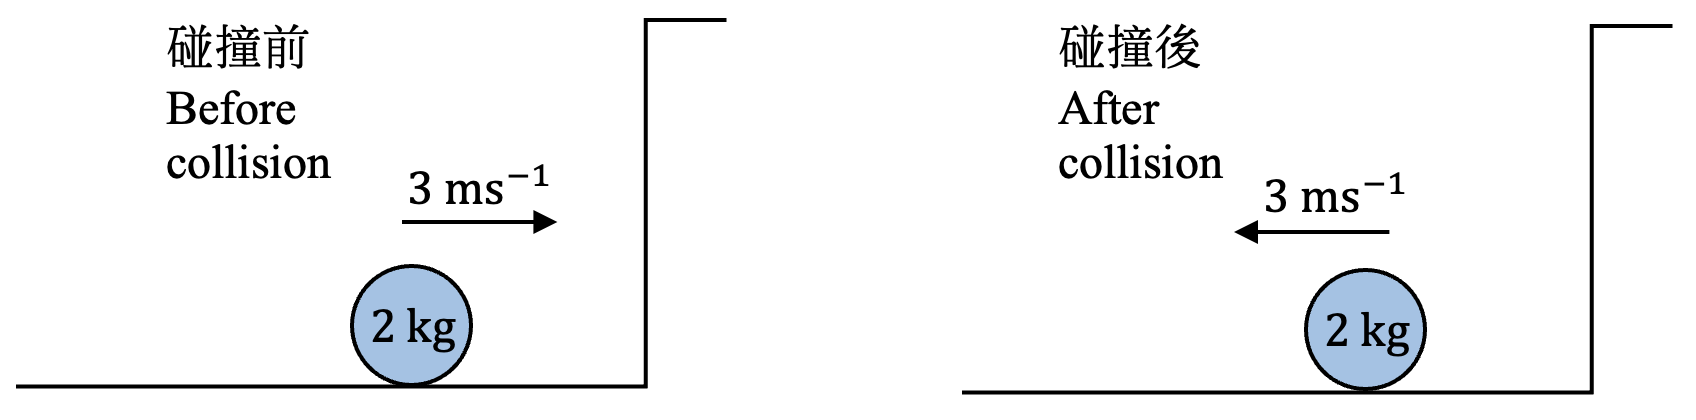
\includegraphics[width=0.66\textwidth]{assets/e26d5e2e.png}
    \par}
    \begin{itemize}
        \item[]\begin{itemize}
                  \item 動量的改變
                  \item[] $\Delta p=mv-mu=(2)(-3)-(2)(3)=\qty{-12}{kg.m.s^{-1}}$
                  \item 動量的改變量值  $=$ \qty{12}{kg.m.s^{-1}}
              \end{itemize}
    \end{itemize}
\end{frame}

\begin{frame}{動量改變Momentum change}
    例 For example:
    {\par\centering
    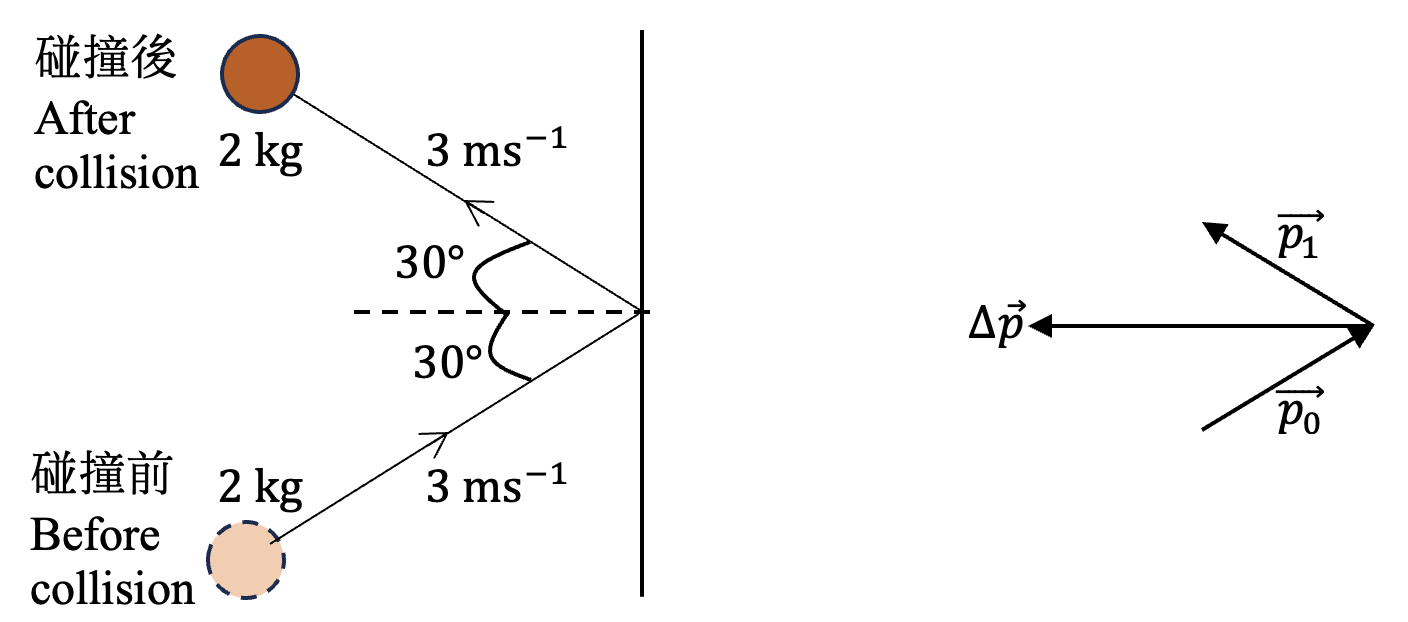
\includegraphics[width=0.66\textwidth]{assets/4c46ae9d.png}
    \par}
    \begin{itemize}
        \item 取向右的方向為正:
        \item 動量的改變只有水平的方向:
        \item[] $\Delta p=m\vec{v}-m\vec{u}=(2)(-3)\cos 30^\circ-(2)(3)\cos 30^\circ=\qty{-10.4}{kg.m.s^{-1}}$
    \end{itemize}
\end{frame}

\begin{frame}{牛頓第二定律Newton's second law}
    \begin{itemize}
        \item 一個系統在外力作用下,必定會有動量變化。
              \begin{itemize}
                  \item [] \textbf{淨力Net force} $F_{net}=ma=\dfrac{m\Delta v}{\Delta t}=\dfrac{\Delta p}{\Delta t}$
              \end{itemize}
    \end{itemize}
    \begin{alertblock}
        {牛頓第二定律的動量版本}
        \begin{equation}
            F_{net}=\frac{\Delta p}{\Delta t}=\frac{mv-mu}{\Delta t}
        \end{equation}
    \end{alertblock}
\end{frame}

\begin{frame}{牛頓第二定律Newton's second law}
    \begin{itemize}
        \item[] \fbox{$F=\dfrac{mu-mu}{t}$}
    \end{itemize}
    {\par\centering
    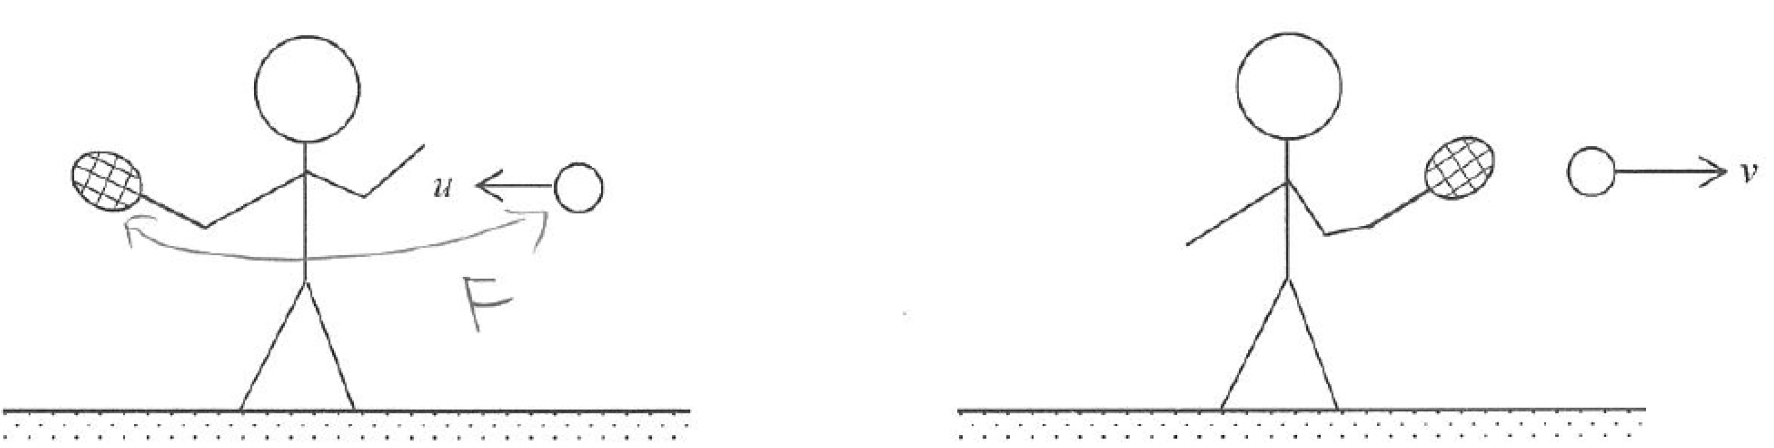
\includegraphics[width=0.66\textwidth]{assets/bc5b866b.png}
    \par}
\end{frame}


\begin{frame}{牛頓第二定律Newton's second law}
    e.g.
        {\par\centering
            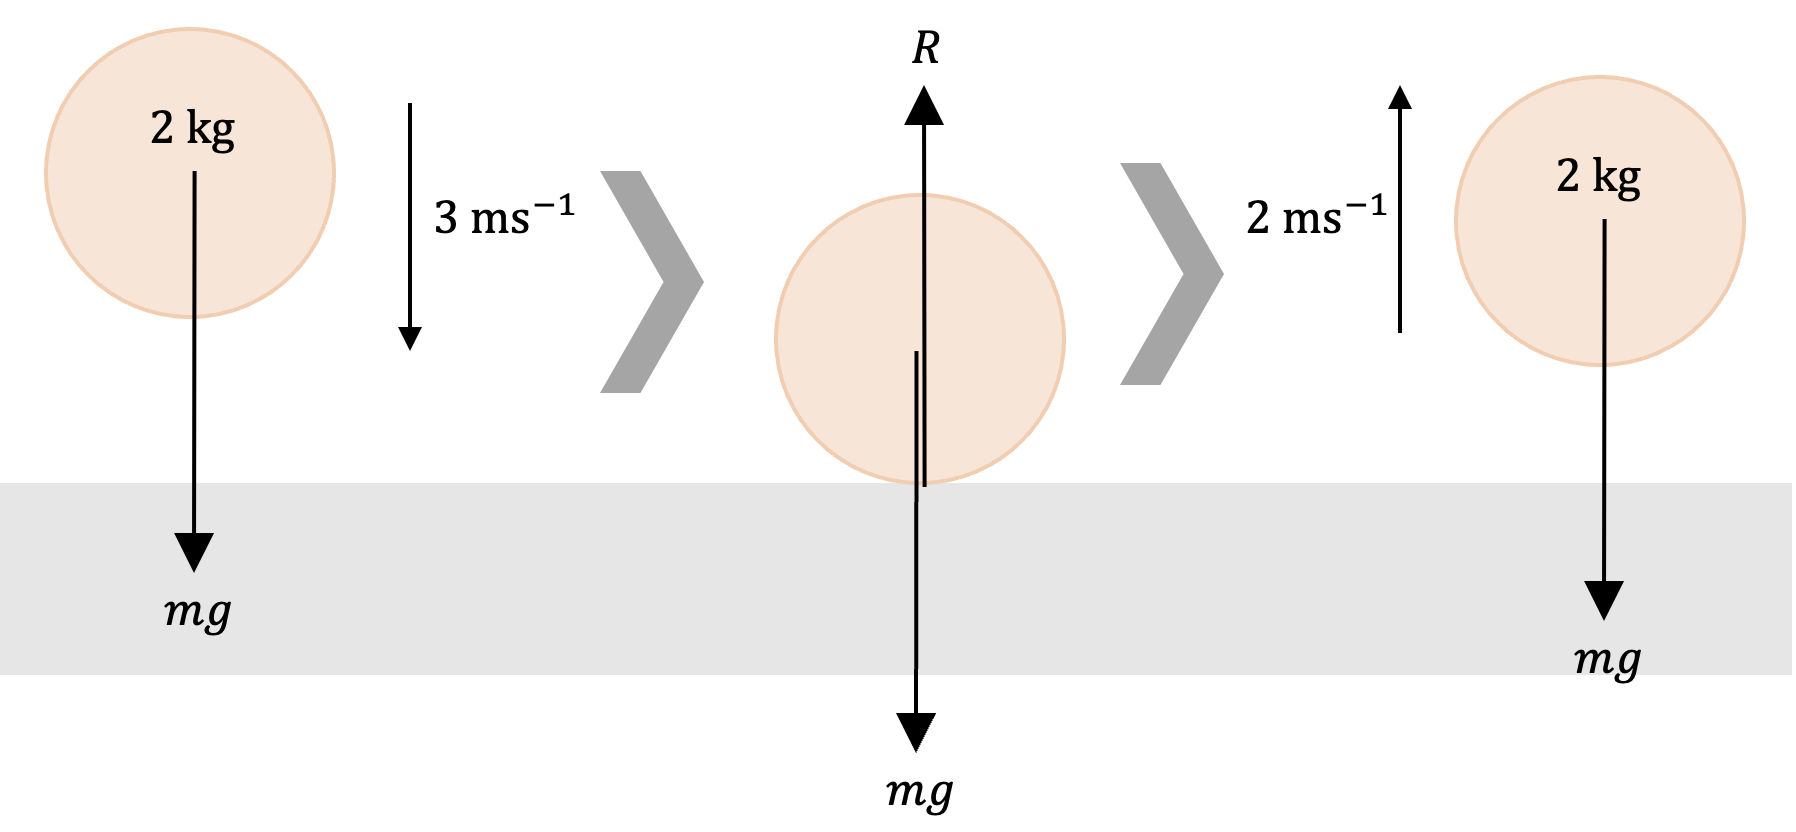
\includegraphics[width=.8\textwidth]{assets/16fb42f7.png}
            \par}



\end{frame}
\begin{frame}{牛頓第二定律Newton's second law}
    己知碰撞時間是 \qty{0.1}{s},求碰撞期間地面施加的力。\medskip
    \begin{columns}
        \column{.5\textwidth}
        \begin{itemize}
            \setlength{\itemsep}{0.6em}
            \item 取向上為正,
            \item []$F_{net}=R-mg = \dfrac{mv-mu}{t}$
            \item []$R-(2)(9.81)=\dfrac{2(2)-2(-3)}{0.1}$
            \item [] $R=\qty{119.62}{N}$
        \end{itemize}
        \column{.5\textwidth}
        \begin{itemize}
            \setlength{\itemsep}{0.6em}
            \item 取向下為正,
            \item []$F_{net}=mg-R = \dfrac{mv-mu}{t}$
            \item []$(2)(9.81)-R=\dfrac{2(-2)-2(3)}{0.1}$
            \item [] $R=\qty{119.62}{N}$
        \end{itemize}

    \end{columns}
\end{frame}


\begin{frame}{連續流動的物體Continuous flowing objects}
    \par
    {\par\centering
        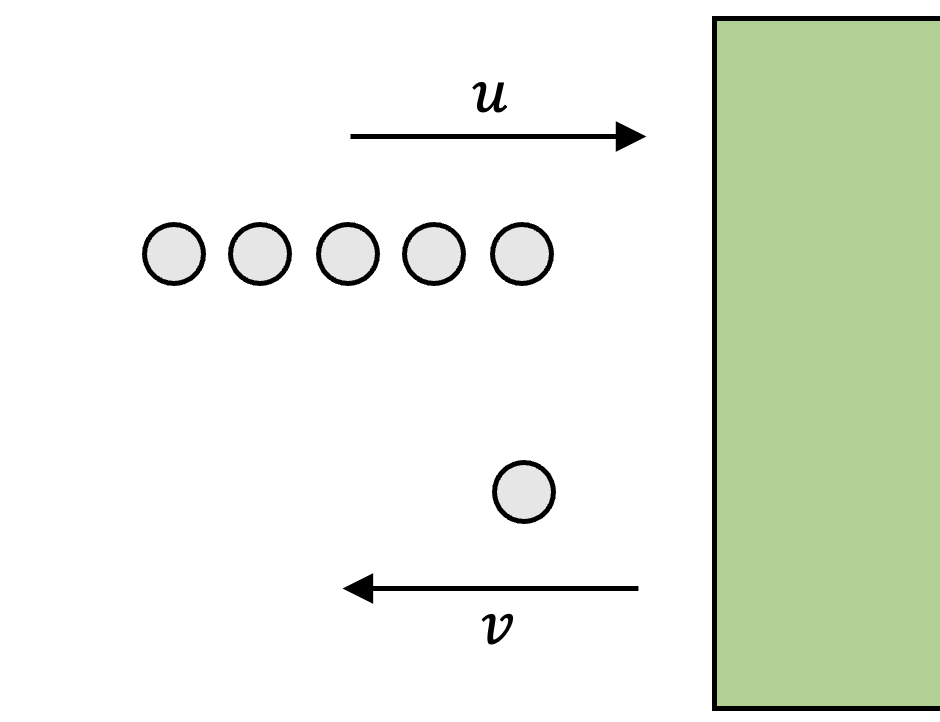
\includegraphics[width=.4\textwidth]{assets/9bad99da.png}
        \par}
    \begin{itemize}
        \item \fbox{$F=\dfrac{m}{t}(v-u)$}
        \item 其中 $\dfrac{m}{t}$是質量的改變/流動速率。
              % \item [] And $\dfrac{m}{t}$ means rate of change of mass/rate of flow of mass.
    \end{itemize}
\end{frame}

\begin{eg}
    \par{\par\centering
        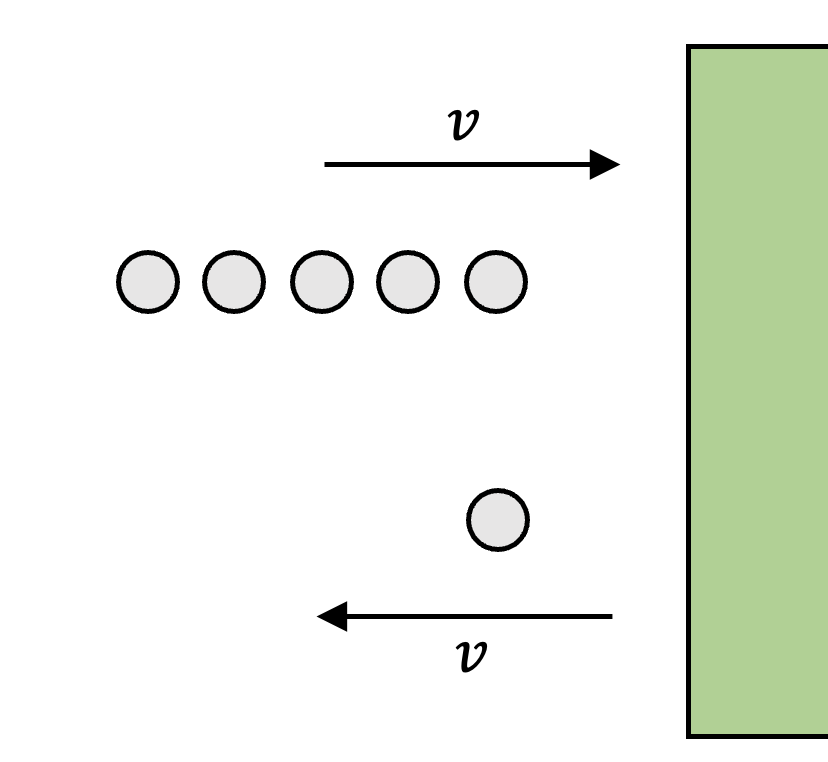
\includegraphics[width=.4\textwidth]{assets/75a1ea9d.png}
        \par}
    子彈以每秒 $n$ 個的發射速率射擊牆壁,每個子彈的質量為 $m$,並以水平速度 $v$ 撞擊牆壁後以相同的水平速度 $v$ 彈回。以下哪個陳述正確?

\end{eg}

\begin{eg}
    \begin{tasks}
        \task [(1)] 子彈的總動量變化是$0$。
        \task [(2)] 子彈每秒的總動量變化是2mnv。
        \task [(3)] 牆壁所受的平均力是2mnv。
    \end{tasks}
\end{eg}

\begin{frame}{動量守恆定律Conservation of momentum}
    \par{\par\centering
        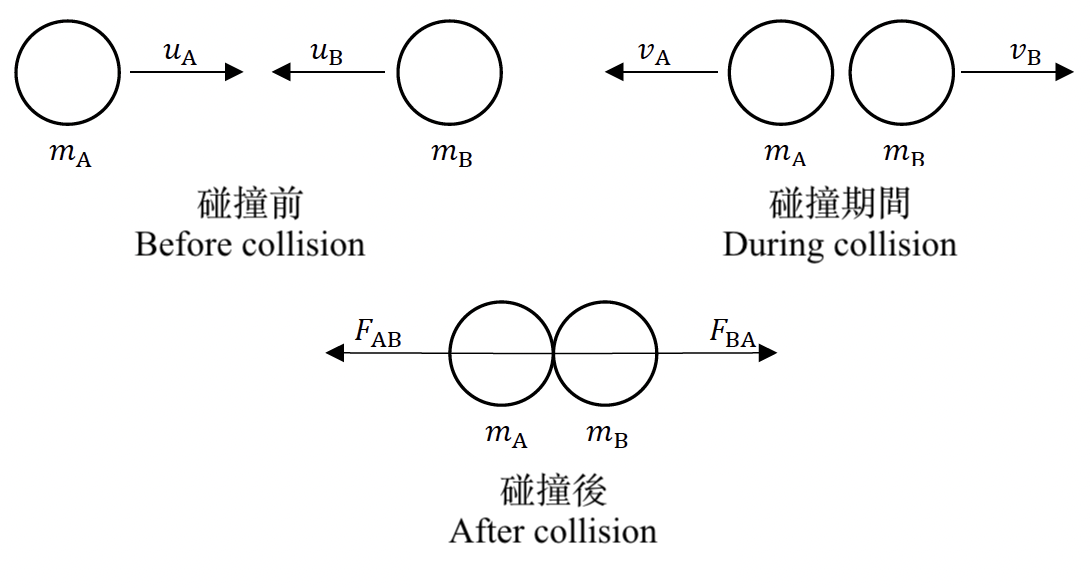
\includegraphics[width=0.8\textwidth]{assets/02c41700.png}
        \par}
\end{frame}
\begin{frame}{動量守恆定律Conservation of momentum}
    \begin{itemize}
        \item 根據牛頓第三定律,
        \item 若沒有外力施於物體,
        \item []$\dfrac{m_A(v_A-u_A)}{t}=-\dfrac{m_B(v_B-u_B)}{t}$
        \item 透過移項可得
        \item []$m_Au_A+m_Bu_B=m_Av_A+m_Bv_B$
    \end{itemize}
\end{frame}
\begin{frame}{動量守恆定律Conservation of momentum}

    \begin{alertblock}
        {動量守恆定律Conservation of momentum}
        \begin{equation}
            m_Au_A+m_Bu_B=m_Av_A+m_Bv_B
        \end{equation}
    \end{alertblock}
    \begin{itemize}
        \item 換言之,一個系統的起始動量總和,等於最終動量總和。
        \item 同樣要注意 $u$ 和 $v$ 也是可以是正或負號。正負號取決於哪個方向取作正。
    \end{itemize}
\end{frame}

\begin{eg}
    質量為 \qty{1000}{kg} 的汽車 P 以 \vel{20} 的速度向前行駛,並與質量為 \qty{1500}{kg} 的汽車 Q 發生正面碰撞。在碰撞前,汽車 Q 以 \vel{10} 的速度朝相反方向行駛。如果兩輛汽車在碰撞後黏在一起,請找出碰撞後它們的共同速度。
\end{eg}

% \begin{eg}
%     一枝火箭最初在太空中靜止不動,火箭接著發生爆炸並分裂為 兩部分。該兩部分沿相反方向運動。若後部分的質量較前部分 的為大,下列哪一項敍述是正確的?
% \end{eg}

\begin{frame}{力和動量的關係線圖Relation graphs between force and momentum}
    \par{\par\centering
        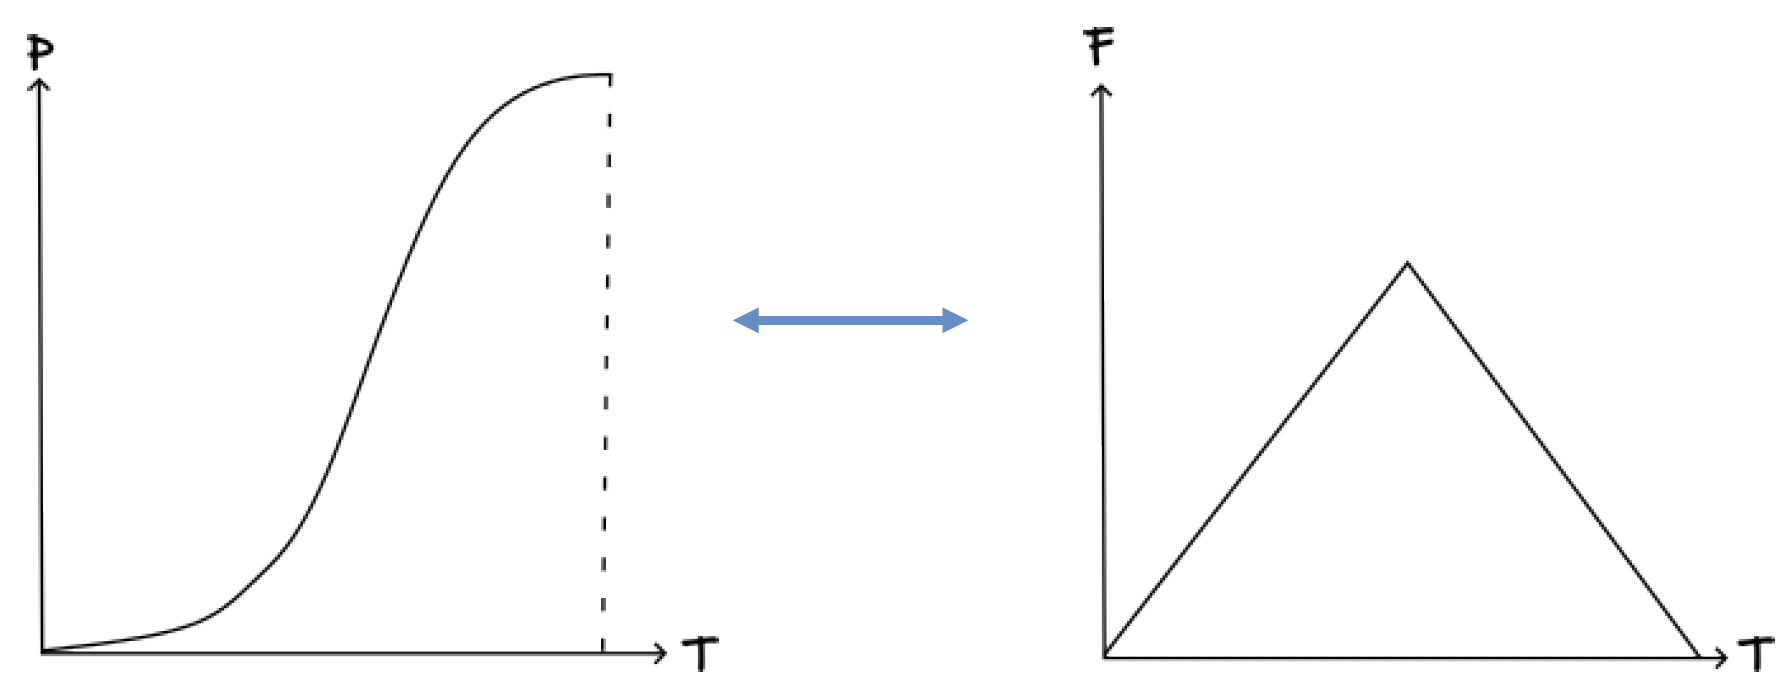
\includegraphics[width=\textwidth]{assets/a8d214ae.png}
        \par}
    \bigskip
    \begin{itemize}
        \item []$\because F=\dfrac{\Delta p}{\Delta t}$,\hspace{1em}$p-t$線圖的斜率$=$$F-t$線圖的值。\\Slope of $p-t$ graphs $=$ value of $F-t$ graphs.
    \end{itemize}
\end{frame}





\begin{frame}{力和動量的關係線圖Relation graphs between force and momentum}
    \par{\par\centering
        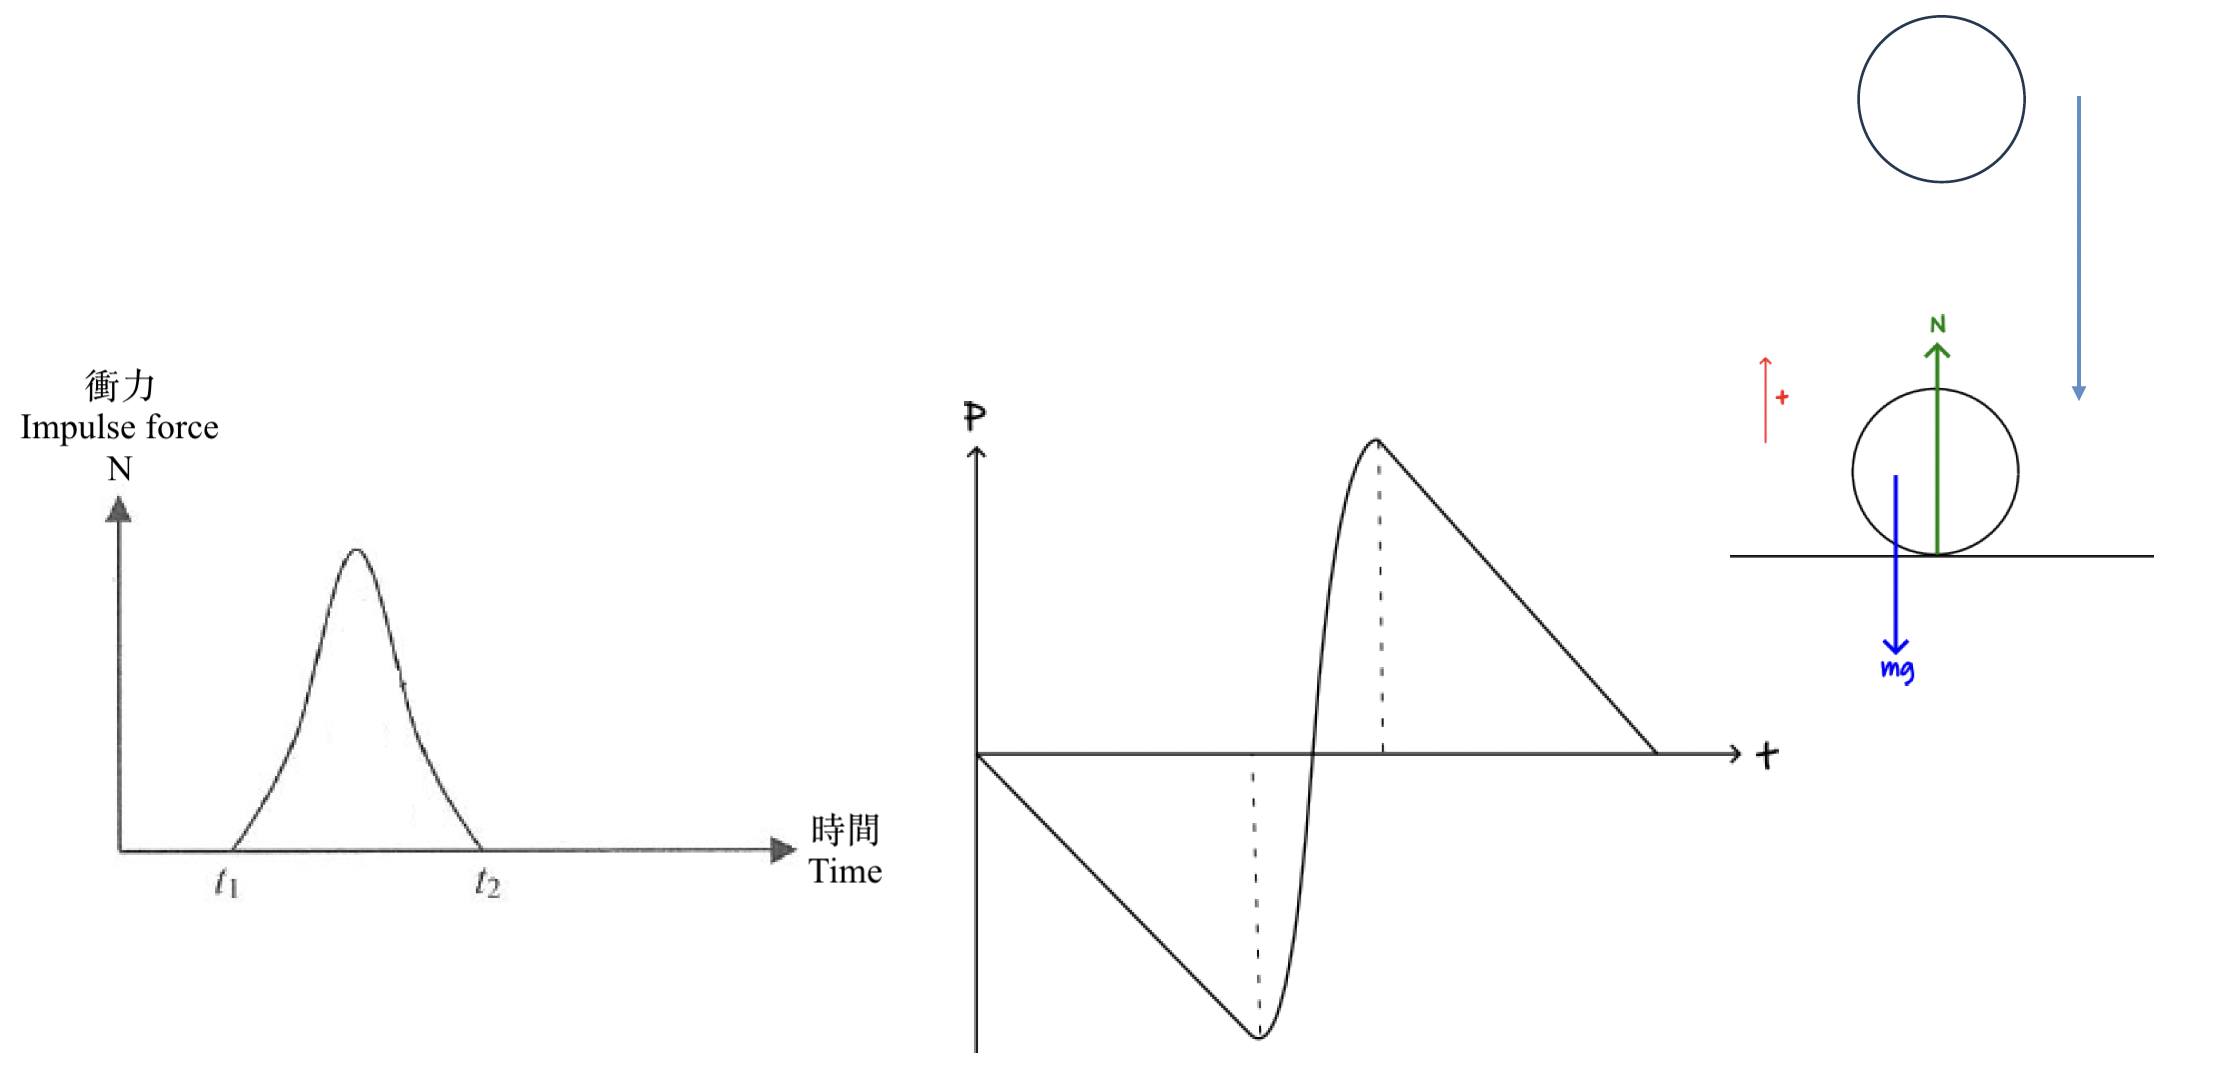
\includegraphics[width=\textwidth]{assets/f231d810.png}
        \par}
\end{frame}


\begin{frame}{力和動量的關係線圖Relation graphs between force and momentum}
    \par{\par\centering
        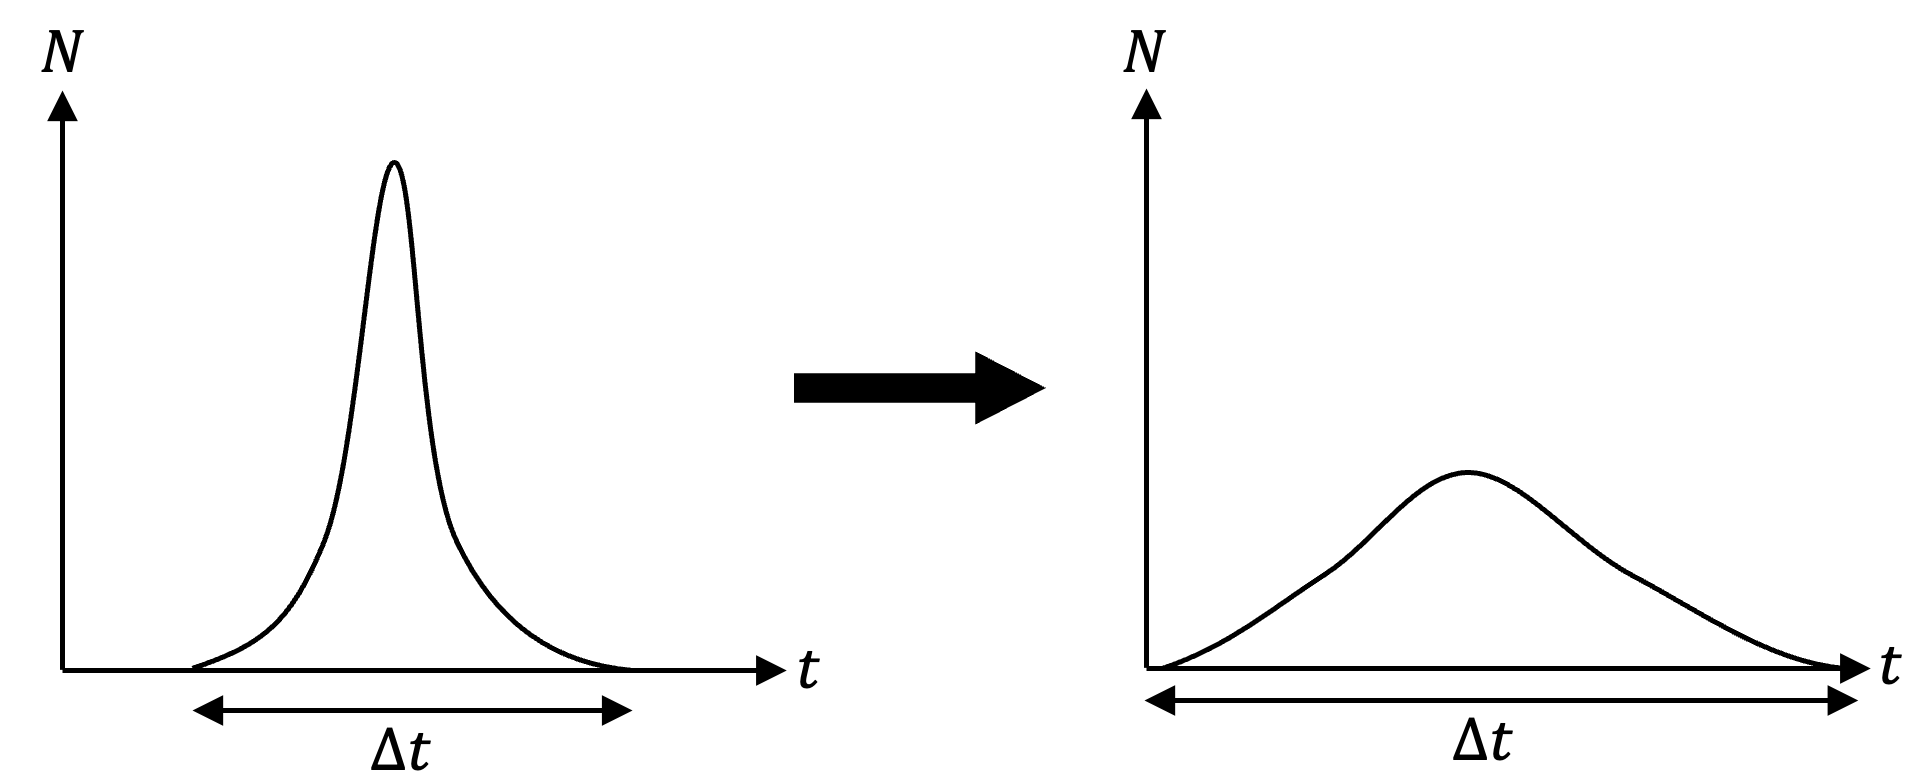
\includegraphics[width=.8\textwidth]{assets/76cc933c.png}
        \par}\bigskip
    \begin{itemize}
        \item 增加撞擊的持續時間$\Delta t$, 可以減少受到的平均衝力 $N$。
    \end{itemize}
\end{frame}

\begin{frame}{力和動量的關係線圖Relation graphs between force and momentum}
    \par{\par\centering
        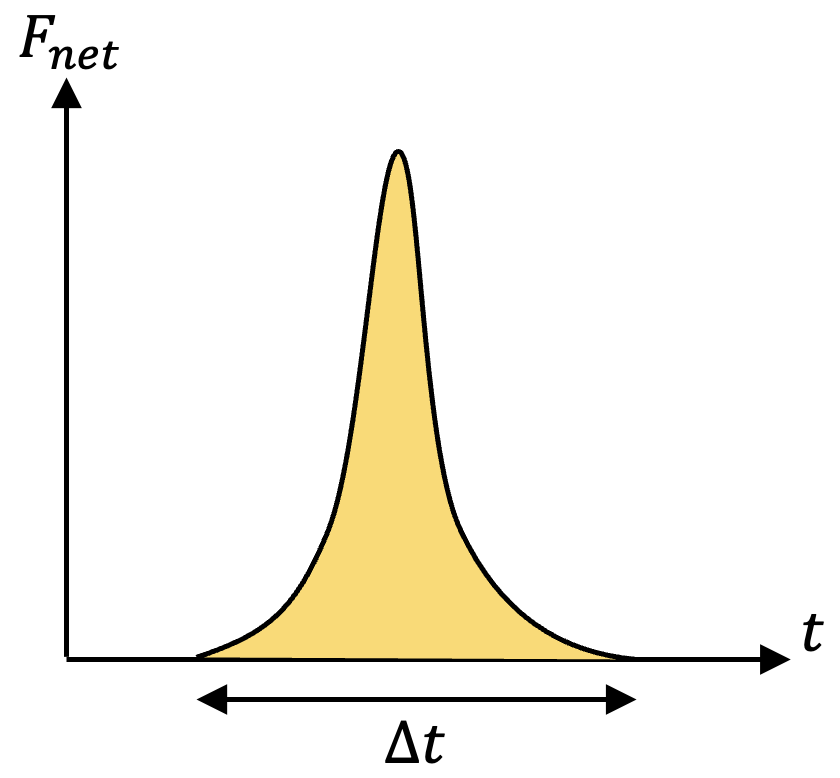
\includegraphics[width=.3\textwidth]{assets/99524ca7.png}
        \par}
    \begin{alertblock}
        {衝量定義Difinition of impulse}
        \begin{itemize}
            \item 衝量Impulse $=mv-mu$
            \item []$=F_{net}-t$ 線圖下的\textbf{面積}\\$=$ \textbf{Area} under $F_{net}-t$ graphs.
        \end{itemize}
    \end{alertblock}

\end{frame}

\begin{frame}{}
    一顆蛋如果從高處掉落並落在硬表面上,很可能會破裂。然而,如果蛋從相同的高度掉落,但落在軟墊上,它可能不會破裂。這是因為使用軟墊時,
    \begin{itemize}
        \item[A.] 蛋在撞擊前的動量變小。
        \item[B.] 蛋撞到軟墊後反彈。
        \item[C.] 蛋在撞擊期間的動量變化率變小。
        \item[D.] 軟墊對蛋的作用力比蛋對軟墊的作用力小。
    \end{itemize}
\end{frame}


% \begin{frame}{汽車上的應用Application to vehicles}
%     \begin{itemize}
%         \item 安全帶具有彈性 $\Rightarrow$ 增加撞擊時間 $\Rightarrow$ 減少碰撞期間的平均撞擊力。
%         \item 安全帶寬度較大 $\Rightarrow$ 增加接觸面積 $\Rightarrow$ 減少對乘客的壓力。
%     \end{itemize}
%     {\par\centering
%     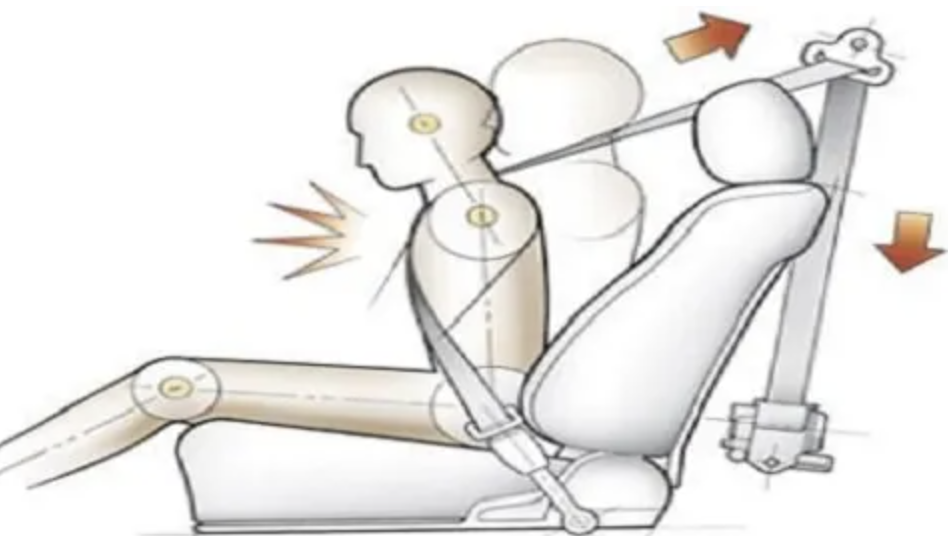
\includegraphics[width=.4\textwidth]{assets/c2b28cb9.png}
%     \par}
% \end{frame}

\begin{frame}{汽車上的應用Application to vehicles}
    \begin{itemize}
        \item 氣袋具有彈性 $\Rightarrow$ 增加撞擊時間 $\Rightarrow$ 減少碰撞期間的平均撞擊力。
    \end{itemize}
    \bigskip
    {\par\centering
        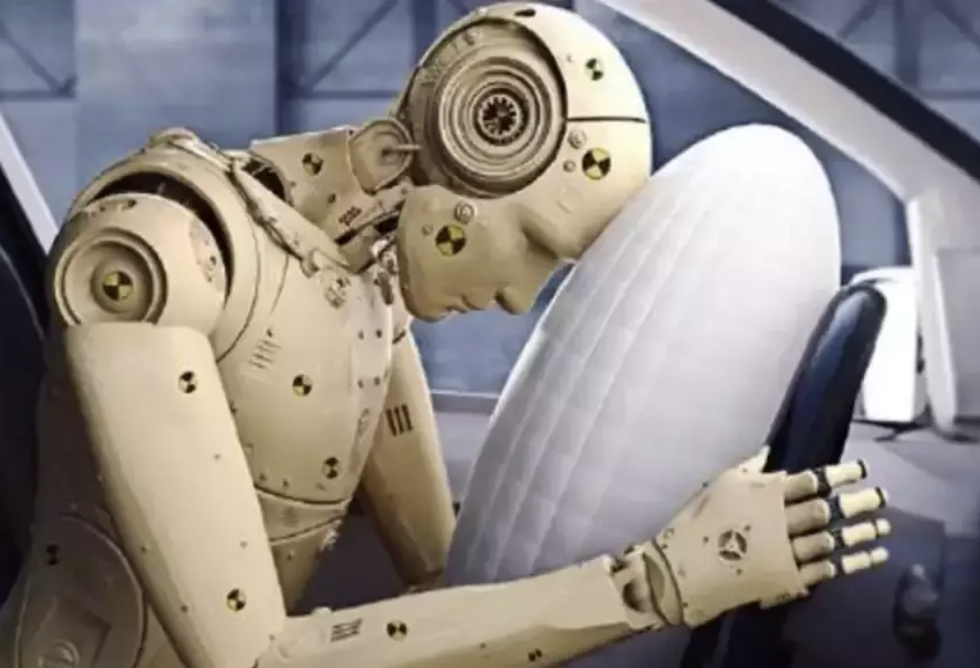
\includegraphics[width=.5\textwidth]{assets/5a24494a.png}
        \par}
\end{frame}

\begin{frame}{汽車上的應用Application to vehicles}
    \begin{itemize}
        \item 汽車泵把具有彈性 $\Rightarrow$ 增加撞擊時間 $\Rightarrow$ 減少碰撞期間的平均撞擊力。
    \end{itemize}\bigskip
    {\par\centering
        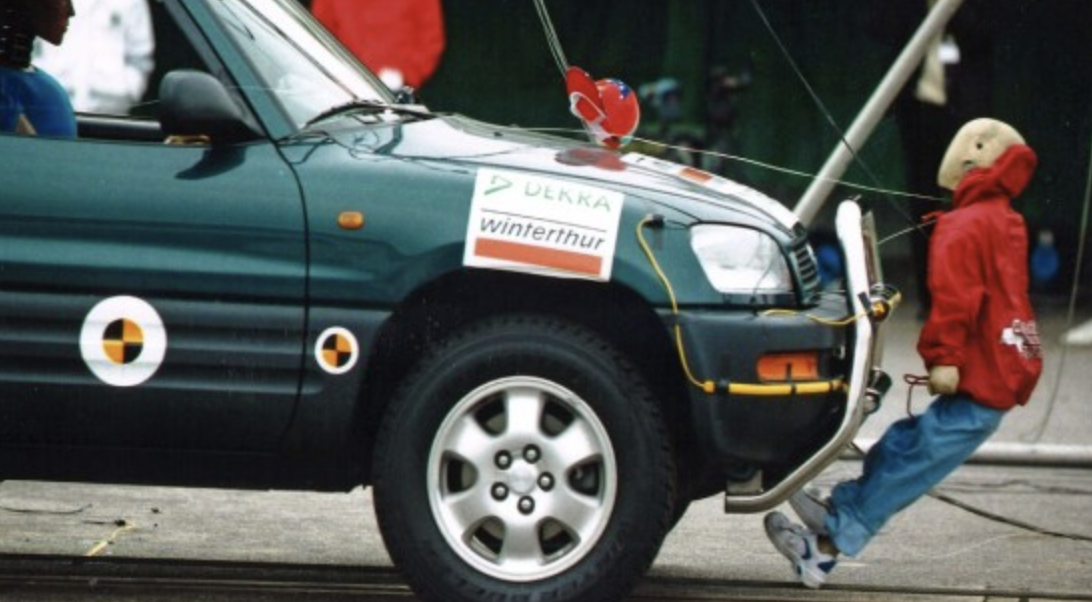
\includegraphics[width=.6\textwidth]{assets/b4012cdb.png}
        \par}
\end{frame}






















































\end{document}